\section{Aspectos Tecnológicos} \label{sect:aspectos_tecnologicos}

En esta sección se presentan las tecnologías y herramientas utilizadas en el desarrollo de la pasantía, así como también algunos términos asociados que son de obligatoria referencia para facilitar al lector la comprensión del contenido subsiguiente. Es necesario hacer una separación entre las tecnologías y herramientas utilizadas para el desarrollo de la aplicación móvil y las asociadas a Tuguia.de con las que se interactuó en el transcurso de la pasantía.

\subsection{Tecnologías Asociadas con la Aplicación Móvil} \label{subsect:Asociadas_movil}

A continuación se presentan las diferentes tecnologías y herramientas involucradas en la construcción de la aplicación Android para Tuguia.de 

\subsubsection{Teléfono Inteligente}

Los teléfonos inteligentes o \textit{smartphones} (nombre en ingles), son teléfonos celulares que ademas de poseer las características habituales de un celular común, permiten acceder a una series de aplicaciones integradas, navegar en Internet, tomar fotografías, grabar vídeos, entre otras funcionalidades que lo asemejan  a una computadora portátil móvil \cite{PCM}.

El objetivo del desarrollo es llevar a Tuguia.de a estos dispositivos.

\subsubsection{Android}

Android es un sistema operativo basado en \textit{Linux}, diseñado en principio para dispositivos móviles con pantalla táctil, es de código abierto y es liberado bajo la licencia Apache; una licencia bastante flexible, que permite que cualquier desarrollador realice aplicaciones y las integre al sistema sin dificultad.

Las aplicaciones nativas se desarrollan, usando el SDK (\textit{Software Development Kit}) y escribiendo la aplicación en lenguaje \textit{Java}. El SDK es un paquete proporcionado directamente por Google que encapsula todas las bibliotecas y herramientas de desarrollo necesarias para crear, probar, y depurar las aplicaciones \cite{ASDK}. Por otro lado existe la alternativa de usar el NDK (\textit{Native Development Kit}) también provisto por Google que permite mediante el uso de lenguajes como \textit{C} y \textit{C++} interactuar directamente con el sistema operativo y crear bibliotecas. Esta última alternativa sólo es recomendada para situaciones específicas donde la aplicación en cuestión realiza cálculos intensivos sobre el \textit{CPU} y debe emplearse sólo cuando el SDK no provee de la funcionalidad deseada\cite{ANDK}.

\paragraph{Arquitectura del Sistema Android}\mbox{}

Gran parte del éxito de este sistema operativo se debe a su arquitectura. En un inicio el sistema fue pensado solo para ser usado en dispositivos móviles, sin embargo, dada su gran capacidad de adaptación, actualmente ademas de ser usado en celulares, también en televisores, reproductores de automóvil, \textit{netbooks} y diversos equipos electrónicos de todo tipo.

Como se observa en la figura \ref{fig:archi} el sistema operativo se desglosa de la siguiente manera:

\begin{figure}[h]
	\begin{center}
		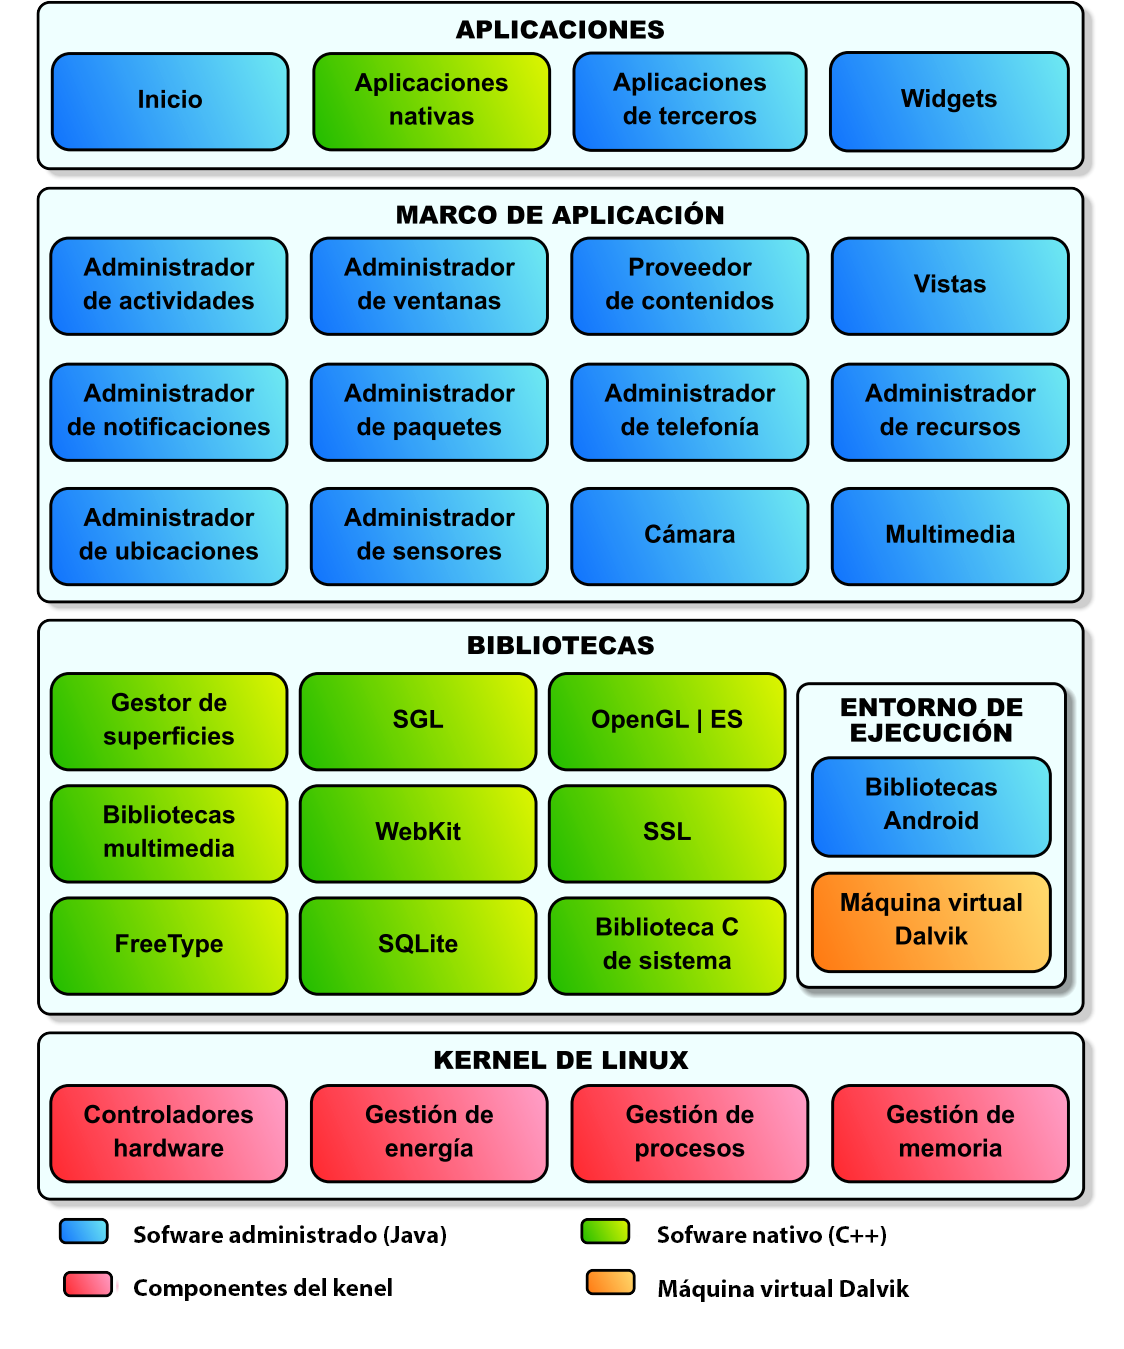
\includegraphics[scale=0.5]{imagenes/pila-android.png}
	\end{center}
	\caption{
		\label{fig:archi}
		Arquitectura del Sistema Operativo Android \cite{AAT}
	}
\end{figure}

\begin{itemize}
\item Aplicaciones: En este nivel se encuentran todas las aplicaciones presentes en el equipo, tanto las instaladas por el usuario como las provistas por el fabricante. Es importante destacar que todas cuentan con la misma capacidad para acceder los servicios que proporciona el sistema operativo. Gracias a esto, se pueden hacerse desarrollos que usen los mismos recursos que usan las aplicaciones nativas. \cite{AAT}.
\item Marco de aplicación: Esta capa esta formada por las diferentes clases que componen el \textit{API} que permiten a las aplicaciones realizar sus funciones, constituyen en el entorno de trabajo que posibilita acceder a los diferentes recursos del dispositivo \cite{AAT}.
\item Bibliotecas: Esta capa se ubica justo sobre el Kernel del sistema operativo y está constituida por un conjunto de bibliotecas escritas en \textit{C} o \textit{C++} que son compiladas para la arquitectura específica del equipo, su función es interactuar con el sistema operativo para acceder a los diferentes recursos gestionados por éste y poner al alcance de las aplicaciones la funcionalidad respectiva.\cite{AAT}. 
\item Entorno de ejecución: Este no se considera una capa como tal puesto que se compone principalmente de un conjunto de bibliotecas que proporcionan la funcionalidad base. El elemento principal de esta sección es la maquina virtual Dalvik que ejecuta cada de las aplicaciones instaladas en el dispositivo \cite{AAT}. 
\item Kernel de Linux: El núcleo del sistema operativo Android es un kernel Linux bastante similar al que puede incluir cualquier distribución de GNU/Linux conocida. En el caso de Android se realizan adaptaciones que permita ajustarse a las características del hardware en el que se ejecutará. Su función principal es proveer una capa de abstracción para el hardware y gestionar los diferentes recursos del teléfono y del sistema operativo \cite{AAT}.
\end{itemize}

\paragraph{Estructura básica de una aplicación Android}\mbox{}

Una actividad es una clase java que contiene todo el código necesario para realizar una determinada tarea. Las actividades son el componente principal de las aplicaciones Android. Una aplicación puede estar compuestas por una o varias actividades que en conjunto desarrollan la funcionalidad de la aplicación. 

Por lo general, las actividades requieren la interacción del usuario. Para lograr esto, la actividad genera en la pantalla una serie de elementos, como campos de textos, botones, formularios, imágenes, entre otros. Estos elementos reciben el nombre de vistas, y son organizados y parametrizados mediante archivos \textit{XML} (\textit{Extensible Markup Language}) llamados \textit{layouts}. A pesar de que la disposición de las vistas es constantes en los archivos XML, una actividad puede modificar totalmente las vistas y sus atributos a tiempo de ejecución.

Cada vez que una aplicación ejecuta una actividad específica, se genera una pila con las actividades relacionadas. Es decir, solo una actividad puede estar en primer plano a la vez, las actividades predecesoras son empiladas en la memoria del teléfono. Cuando una actividad termina o el usuario presiona el botón atrás se pasa la siguiente en la pila. La figura \ref{fig:backstack} ilustra el comportamiento.

\begin{figure}[h]
	\begin{center}
		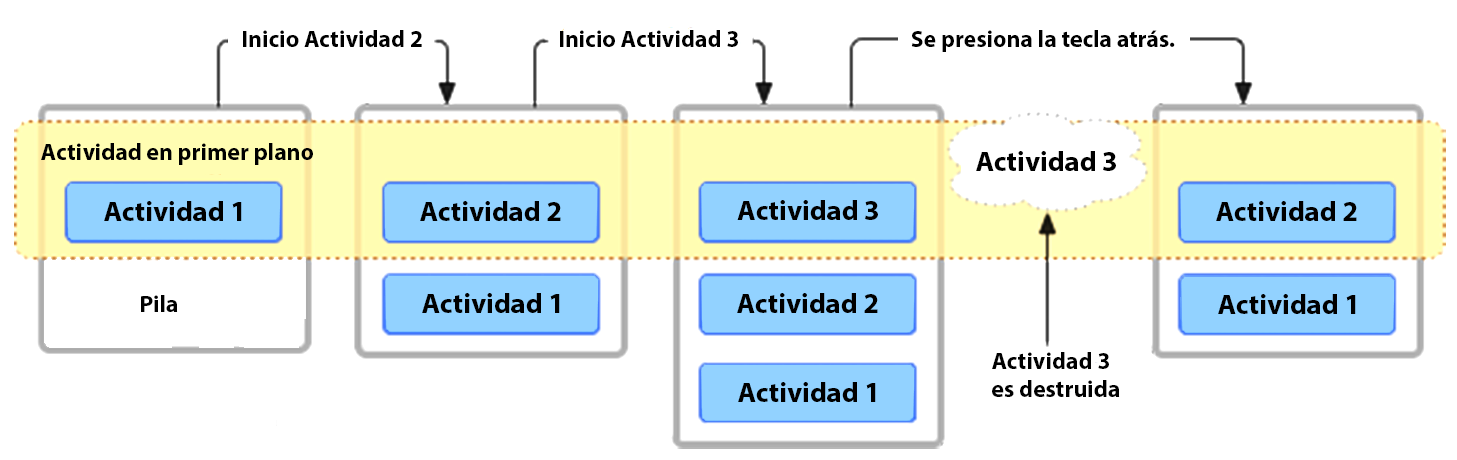
\includegraphics[scale=0.7]{imagenes/diagram_backstack.png}
	\end{center}
	\caption{
		\label{fig:backstack}
		Interacción y flujo de Actividades en Android \cite{TBS}
	}
\end{figure}

\paragraph{\textit{SQLite}} \mbox{}

\textit{SQLite} es un manejador de base de datos relacional de código abierto, usa sintaxis \textit{SQL} (\textit{Structured Query Language}), implementa transacciones y soporta \textit{triggers}, En \textit{SQLite} el conjunto de la base de datos (definiciones, tablas, índices, y los propios datos), son guardados como un sólo archivo y el requerimiento de memoria durante la ejecución es bastante bajo aprox 250KByte, lo que hace que este manejador sea fácilmente embebido en otros sistemas. Gracias a estas características el sitema Android cuenta con una base de datos \textit{SQLite} integrada y de fácil acceso para las aplicaciones.

\subsubsection{Eclipse}

Eclipse es un entorno integrado de desarrollo (\textit{Integrated development environment}, IDE por sus siglas en ingles) gratuito y de código abierto. Está escrito en \textit{Java} con el objetivo de realizar aplicaciones en este lenguaje. sin embargo permite la integración con otros como \textit{C, C++, Ada, Haskell, PHP, Python, Ruby}.

Este ambiente de trabajo es recomendado por Google para la construcción de aplicaciones Android, ya que a través de la instalación de un \textit{plugin} distribuido en el sitio oficial, permite integrar en este entorno el soporte necesario para emplear diversas herramientas específicas para Android que facilitan el desarrollo, cuenta con plantillas para las diversas clases básicas, instrumentos para el análisis del desempeño de la aplicación y facilidades para la gestión de emuladores que permiten simular \textit{smartphones} de diversas características y funciones.

Por ser el entorno oficial de desarrollo cuenta con un amplio soporte y el respaldo de la comunidad, por lo que es el ambiente escogido para el desarrollo de Tuguia.de móvil.

\subsection{Tecnologías Asociadas con Tuguia.de} \label{subsect:Asociadas_movil}

Durante el desarrollo del proyecto, fue necesario incidir directamente sobre el API de Tuguia.de para agregar funcionalidad, hacer mejoras y ajustes necesarios para garantizar un adecuado desarrollo de la aplicación móvil, las tecnologías implicadas en este proceso serán descritas a continuación.

\subsubsection{Drupal}

Drupal es un marco de gestión de contenidos de código abierto escrito en lenguaje \textit{PHP}. En otra palabras, es una interfaz de programación de aplicaciones para crear sistema de gestión de contenidos (\textit{Content Managemement System}, CMS por su siglas en ingles). Una instalación base del sistema o \textit{el núcleo de Drupal} provee los elementos necesarios para el funcionamiento de un CMS básico, sin embargo, la funcionalidad se puede extender mediante la integración y desarrollo de módulos o paquetes\cite{TV10}.

El sitio Tuguia.de fue desarrollado con esta herramienta y mediante la instalación, configuración y elaboración de varios módulos fue implementado un API que permite mediante peticiones HTTP (\textit{Hypertext Transfer Protocol})gestionar el contenido del portal.

\subsubsection{Apache Solr}

Apache Solr es una plataforma de búsqueda de alto desempeño para sitios web, es de código abierto, esta escrita en lenguaje \textit{Java} y se basa en la biblioteca \textit{Apache Lucene} \cite{APS}. Apache Solr opera como un servicio separado del servidor web y la base de datos, puede incluso llegar a requerir un servidor dedicado para su operación. 

De forma sencilla el funcionamiento de Apache Solr puede ser descrito de la siguiente manera: Mediante archivos \textit{XML} se especifican los contenidos que serán indexados para su posterior búsqueda, estos indices pueden ser vistos como una lista de palabras en la que cada palabra en la lista posee una referencia hacia los documentos que la contienen, cuando se realiza una consulta a Apache Solr se ejecuta una búsqueda sobre las listas y se retornan los elementos que cumplan con el criterio establecido en la consulta.

Apache Solr permite realizar búsquedas de texto (\textit{Full-Text Search}) por palabra clave de forma similar al buscador de Google y tiene la capacidad para manejar búsquedas geoespaciales, por lo que en Tuguia.de, es ésta la herramienta elegida para realizar las búsquedas y es integrada a Drupal mediante un módulo de código abierto ampliamente configurable.  
